\documentclass[10pt, a4paper, twosize]{article}
%\documentclass[12pt, a4paper, twoside]{book}

\usepackage{helvet}
\usepackage{hyperref}
\usepackage{graphicx}
\usepackage{listings}
\usepackage{textcomp}
\usepackage[
	a4paper,
	outer=2cm,
	inner=4cm,
	top=2cm,
	bottom=2cm
]{geometry}
\usepackage{float}
\usepackage{tabularx}
\usepackage[disable]{todonotes}
\usepackage{color, soul}
\usepackage{amsmath}
\usepackage{algorithmicx}
\usepackage[noend]{algpseudocode}
\usepackage{algorithm}
\usepackage{framed}
\usepackage{subcaption}
\usepackage{titlepic}
\usepackage{fancyhdr}
\usepackage[simplified]{styles/pgf-umlcd}
\usepackage{shorttoc}
\usepackage{url}
\usepackage{paralist}
\usepackage{verbatim}

\definecolor{grey}{rgb}{0.9, 0.9, 0.9}
\definecolor{dkgreen}{rgb}{0,0.6,0}
\definecolor{dkred}{rgb}{0.6,0,0.0}

\lstdefinestyle{DOS}
{
    backgroundcolor=\color{black},
    basicstyle=\scriptsize\color{white}\ttfamily,
    stringstyle=\color{white},
    keywords={}
}

\lstdefinestyle{makefile}
{
    numberblanklines=false,
    language=make,
    tabsize=4,
    keywordstyle=\color{red},
    identifierstyle= %plain identifiers for make
}

\lstset{
  language=Java,                % the language of the code
  basicstyle=\footnotesize\ttfamily,
  numbers=left,                   % where to put the line-numbers
  stepnumber=1,                   % the step between two line-numbers. If it's 1, each line
  numbersep=5pt,                  % how far the line-numbers are from the code
  backgroundcolor=\color{white},      % choose the background color. You must add \usepackage{color}
  showspaces=false,               % show spaces adding particular underscores
  showstringspaces=false,         % underline spaces within strings
  showtabs=false,                 % show tabs within strings adding particular underscores
  frame=single,                   % adds a frame around the code
  rulecolor=\color{black},        % if not set, the frame-color may be changed on line-breaks within not-black text (e.g. comments (green here))
  tabsize=2,                      % sets default tabsize to 2 spaces
  captionpos=b,                   % sets the caption-position to bottom
  breaklines=true,                % sets automatic line breaking
  breakatwhitespace=false,        % sets if automatic breaks should only happen at whitespace
  keywordstyle=\color{blue},          % keyword style
  commentstyle=\color{dkgreen},       % comment style
  stringstyle=\color{dkred},         % string literal style
  columns=fixed,
  extendedchars=true,
  frame=single,
}

%\renewcommand{\chaptername}{Topic}

% New definitions
\algnewcommand\algorithmicswitch{\textbf{switch}}
\algnewcommand\algorithmiccase{\textbf{case}}
\algnewcommand\algorithmicassert{\texttt{assert}}
\algnewcommand\Assert[1]{\State \algorithmicassert(#1)}%
% New "environments"
\algdef{SE}[SWITCH]{Switch}{EndSwitch}[1]{\algorithmicswitch\ #1\ \algorithmicdo}{\algorithmicend\ \algorithmicswitch}%
\algdef{SE}[CASE]{Case}{EndCase}[1]{\algorithmiccase\ #1}{\algorithmicend\ \algorithmiccase}%
\algtext*{EndSwitch}%
\algtext*{EndCase}%

\pagestyle{fancy}
\fancyhf{}
\fancyhead[RO, LE]{\small \rightmark}
\fancyfoot[RO, LE]{\small \thepage}

\begin{document}

%\frontmatter

\begin{titlepage}
\vspace*{5cm}
\begin{center}

\includegraphics[width=.5\textwidth]{images/EdNapUniLogoCMYK}~\\[1cm]

\textsc{\Large Edinburgh Napier University}\\[1.5cm]

\textsc{\LARGE \bfseries SET08101 Web Tech}\\[0.5cm]

\hrulefill \\[0.4cm]
{\huge \bfseries Lab 10 - Datastores \& Persistence \\[0.4cm] }
\hrulefill \\[1.5cm]

\begin{minipage}{0.4\textwidth}
\begin{flushleft} \large
\textbf{Dr Simon Wells} \\
\end{flushleft}
\end{minipage}

\vfill

\end{center}
\end{titlepage}

%\shorttoc{Overview}{0}

%\setcounter{tocdepth}{2}
%\cleardoublepage
%\tableofcontents
%\listoffigures
%\listofalgorithms
%\addtocontents{toc}{~\hfill\textbf{Page}\par}

%\mainmatter

%\input{sections/labs/04_ui}

\section{Aims}
\paragraph{} At the end of the practical portion of this topic you will be able to:

\begin{itemize}
\item Persist data to the filesystem
\item Use SQLite3 to persist data using a relational database
\item Use mLab to persist data in a cloud version of MongoDB
\end{itemize}


%\begin{framed}
%{\bf{NOTICE:}  }
%\end{framed}


\section{Activities}

\paragraph{} If we want a website to be dynamic, to let user's interact with it beyond just reading static data, then there is a good chance that we'll want to save some of that data. We have a number of strategies to achieve this. We'll take two main approaches to persisting our data, firstly on the client side, and then on the server side. 

\paragraph{} For the client side we'll look at ways to store data using the browser; cookies and web-storage%, and the nascent Indexed DB.

\paragraph{} For the Server-side we also have three approaches, firstly using the filesystem, a simple, straightforward, and robust solution. Secondly we'll try a traditional relational database, then lastly we'll look at a cloud-based version of a NoSQL datastore.

\paragraph{} Data storage is a huge topic so this lab only really scratches the surface. However, you should, by the end, feel comfortable with persisting data on the server or client, and should be building some skills in deciding which approach to take depending upon the problems that you are presented with.

\subsection{Cookies}
\paragraph{} We can create cookies from JavaScript. It's not the only way, but it is a good method to get started. You can do the following exercises from the Javascript console in your browser, first ensuring that you have cookies enabled. Cookies have a really simple JavaScript API. For the most part just using a call to document.cookie is sufficient to create, retrieve, update, and delete a cookie.

\paragraph{} Enter the following into the console, replacing ``your name'' with your actual name.
\begin{lstlisting}
    document.cookie = "username=your name";
\end{lstlisting}
\paragraph{} This will add the double-quoted content to the ``cookie string'' for the current page.


\paragraph{} To retrieve our cookie we need to create a variable and then call document.cookie which returns the cookie string. In the next example we will do so then print out the variable using console.log()
\begin{lstlisting}
    var x = document.cookie;
    console.log(x);
\end{lstlisting}
\paragraph{} We can also set an expiry date for a cookie, for example:

\begin{lstlisting}
document.cookie = "password=secret; expires=Thu, 18 Dec 2019 12:00:00 UTC"; 
\end{lstlisting}

\paragraph{} After the expiry date, that particular key \& value pair will be deleted.

\paragraph{} If we repeat the retrieval of our cooke from above, we'll notice that our password key has been appended to hte previous string so both username and password are stored in the same cookie. This is because there is just one cookie string for each page. So to retrieve a particular key we need to pull apart the cookie using JavaScript to retrieve the specific key that we are interested in.

\paragraph{} For example, to retrieve just the value for the username we could create a function that searches the cookie string for the supplied cookie\_name, e.g.
\begin{lstlisting}
function getCookie(cookie_name)
{
    var name = cookie_name + "=";
    var decodedCookie = decodeURIComponent(document.cookie);
    var ca = decodedCookie.split(';');
    for(var i = 0; i <ca.length; i++)
    {
        var c = ca[i];
        while (c.charAt(0) == ' ') 
        {
            c = c.substring(1);
        }
        if (c.indexOf(name) == 0) 
        {
            return c.substring(name.length, c.length);
        }
    }
    return "";
}
\end{lstlisting}

\paragraph{} We can then use our function to retrieve a specific value from the cookie, for example, the username:

\begin{lstlisting}
console.log(getCookie("username"));
\end{lstlisting}

\paragraph{} Deleting a cookie is achieved by setting an expiry date that is in the past, for example:
\paragraph{} 
\begin{lstlisting}
document.cookie = "username=; expires=Thu, 01 Jan 1970 00:00:00 UTC;";
\end{lstlisting}
\paragraph{}

\paragraph{} To update a value stored in a cookie you merely replace the existing key with the new kvalue, for example, here we just set a new username with an updated value which will replace the existing value:
\begin{lstlisting}
document.cookie = "username=Carol Danvers;";
\end{lstlisting}

\paragraph{} Your cookies should probably not live forever, it is good practise to set an expiry date which is a reasonable length of time into the future. To make it easier to program, a nice way to do this is to use a function, for example, this one will create a cookie using the supplied key and value and will set an expiry date based upon the supplied value for the number of days.

\begin{lstlisting}
function setCookie(name, value, expiry)
{
    var d = new Date();
    d.setTime(d.getTime() + (expiry*24*60*60*1000));
    var expires = "expires="+ d.toUTCString();
    document.cookie = name + "=" + value + ";" + expires;
}
\end{lstlisting}

\paragraph{} Now create a simple site using HTML, CSS, \& JS that uses cookies to persist some data. A good place to start is to create a simple form that asks some questions about the user. stores the responses in a cookie, then uses the data in the cookie to personalise a message to the user. For example, asking a user what their name is, then whether they are happy or sad and respond with something appropriate that is personalised to them.

\subsection{Web Storage}

\paragraph{} This option provides more space for your site to store data on the client. The amount of space is browser specific, and the API is only supported by newer browsers, so you'll have to check first, in code, whether web storage is supported.

\paragraph{} The basic idea with web-storage is that you can store keys and values. Both keys and values are always strings, so you may have to do some type conversion for some of your variables. If you have JSON objects, then you can store these by converting them to a string using the JSON.stringify function. Thera are two types of web-storage available, localStorage and sessionStorage. The main difference is that sessionStorage is only available whilst the current window is open and is deleted afterwards, i.e. once your current session is over. However data stored in local storage will be available for ever unless explicitly deleted, for example, by your webapp, or by the user clearing all local data, reformatting their drive, etc.

\paragraph{} 

\begin{lstlisting}
function storageAvailable(type)
{
    try
    {
        var storage = window[type],
            x = '__storage_test__';
        storage.setItem(x, x);
        storage.removeItem(x);
        return true;
    }
    catch(e)
    {
        return e instanceof DOMException && (
            e.code === 22 ||
            e.code === 1014 ||
            e.name === 'QuotaExceededError' ||
            e.name === 'NS_ERROR_DOM_QUOTA_REACHED') &&
            storage.length !== 0;
    }
}
\end{lstlisting}
\paragraph{} In this we attempt to use the storage API and then catch any exceptions that are thrown. Even if storage is available, there are reason why it might not be usable, either due to local settings, such as privacy settings, the way that private browsing works (if you are in a private browsing window then you might have local storage available but the amount of space to store anything in is set to zero), or because you've already filled it up.

\paragraph{} We can call our storageAvailable function with the value ``localStorage'' or ``sessionstorage'' to see which is available to use.
\begin{lstlisting}
if (storageAvailable('localStorage'))
{
    // We can do something with the localStorage...
}
else 
{
    // Have to come up with an alternative way to store data
}
\end{lstlisting}

\paragraph{} We can then actually add data to the storage using the setItem function, for example,
\begin{lstlisting}
localStorage.setItem('name','simon');
\end{lstlisting}
\paragraph{} Checking whether something has been set can be quite useful. We can achieve that like this using the getItem function (we assume that we, as programmers, will know which keys our web pages will have set):

\begin{lstlisting}
if(localStorage.getItem('name')) {console.log("set");}
\end{lstlisting}

\paragraph{} We can also retrieve that data using the getItem function, for example, let's retrieve what we just stored and display it:
\begin{lstlisting}
var myname = localStorage.getItem('name');
console.log(myname);
\end{lstlisting}
\paragraph{}



\begin{comment}
\subsection{Indexed DB}
\paragraph{} Another browser API, this time much more complex, and aimed at providing a full client side database for use by the browser and more advanced web-applications. Think of cookies, webstorage, and Indexed DB as a hierarchy of increasing power and complexity, from very limited data storage with a restricted API in cookies, through more space, longer persistence, and a slightly more complex API with web storage, right through to Indexed DB which can store significant volumes of data with less restrictions than are found with web-storage. Because this is more complex, and becaues IndexedDB is currently a candidate standard which might yet be enhanced or surpassed, we'll only take a brief look at it now.

\paragraph{} We can check whether our browser has support for Indexed DB using something like this:
\begin{lstlisting}
if (('indexedDB' in window))
{
    console.log('This browser supports IndexedDB');
}
\end{lstlisting}
\paragraph{}

\paragraph{} 
\begin{lstlisting}
(function()
{
  'use strict';

  //check for support
  if (!('indexedDB' in window)) {
    console.log('This browser doesn\'t support IndexedDB');
    return;
  }

  var dbPromise = indexedDB.open('test-db1', 1);

})();
\end{lstlisting}
\paragraph{}



\paragraph{} 
\begin{lstlisting}

\end{lstlisting}
\paragraph{}



\paragraph{} 
\begin{lstlisting}

\end{lstlisting}
\paragraph{}
\end{comment}



\subsection{Filesystem}
\paragraph{} Whilst JS usually has little support for input and output which is all handled by the browser environment in which the JS runs, Node gives us other opportunities. Saving files to the file system is a useful and simple technique that can lead to robust, reliable sites and good performance. We can use the \emph{fs} Node module. We'll need to install fs using NPM first, e.g.

\begin{lstlisting}[style=DOS]
    npm install fs
\end{lstlisting}

\paragraph{} Now we can use it from code, for example, put the following code into a file called \emph{filesystem.js}:

\begin{lstlisting}
var http = require("http"),	fs = require("fs");

http.createServer(function (request, response) {
	request.on("end", function () {
		fs.readFile("test.txt", 'utf-8', function (error, data) {
			response.writeHead(200, {
				'Content-Type': 'text/plain'
			});
			data = parseInt(data) + 1;
			fs.writeFile('test.txt', data);
			response.end('This page was refreshed ' + data + ' times!');
		});
	});
}).listen(5000);
\end{lstlisting}

\paragraph{} We read and write files by using calls to the fs.readFile() and fs.writeFile() methods respectively. Note that you will need to create the file \emph{test.txt} in the same folder as filesystem.js before running it. When you run the file you should be able to access it at \url{http://localhost:5000}

\subsection{SQLite3}
\paragraph{} A drawback of the file system as a way to persist your data is that performing \emph{ad hoc} queries of your data is more difficult. Unless you have developed a plan for searching all your files, or have a strategy for finding data across multiple files, it can be difficult to find specific things that you need. Databases generally provide ways to manage searching through your data and can be useful when the size of your data becomes large. However, they also add great complexity to your design compared with a site that merely reads and writes files on the local filesystem. For small amounts of data they can be overkill and you should seldom reach for a database as your solution to data storage without a positive reason why you are doing so.

\paragraph{} Rather than installing a large SQL-based datastore manager we will use SQLite3. This is an efficient, embedded datastore, that is available on most platforms, and roundly regarded as a reliable, well-engineered. It also happens to perhaps be the most widely deployed datastore on the planet embedded within many operating systems, email clients, and web browsers as a way to reliably persist data.

\paragraph{} Create a folder called counter then navigate into it. We can install SQLite3 using NPM:

\begin{lstlisting}[style=DOS]
    npm install sqlite3
\end{lstlisting}

\paragraph{} Once the SQLite3 package is installed you can use it from Node. First however you will need to create a database file. Create a file called count.db in counter folder. This will be the file that SQLite3 uses to store data from our counter node app. Note that the node app doesn't create this file for you and will throw an error if it can't find the nominated database file. You can write some setup code if you like that will create this file for you but that is left as an exercise...

\begin{lstlisting}
var path = require('path');
var dbPath = path.resolve(__dirname, 'count.db')

var sqlite3 = require('sqlite3').verbose();
var db = new sqlite3.Database(dbPath);

db.serialize(function() {
    db.run("CREATE TABLE IF NOT EXISTS counts (key TEXT, value INTEGER)");
    db.run("INSERT INTO counts (key, value) VALUES (?, ?)", "counter", 0);
});



var express = require('express');
var counterapp = express();

counterapp.get('/data', function(req, res){
    db.get("SELECT value FROM counts", function(err, row){
        res.json({ "count" : row.value });
    });
});

counterapp.post('/data', function(req, res){
    db.run("UPDATE counts SET value = value + 1 WHERE key = ?", "counter", function(err, row){
        if (err){
            console.err(err);
            res.status(500);
        }
        else {
            res.status(202);
        }
        res.end();
    });
});


counterapp.listen(5000);

console.log("Submit GET or POST to http://localhost:5000/data");

\end{lstlisting}


\paragraph{} Use curl to POST to the api:

\begin{lstlisting}[style=DOS]
    curl -X POST localhost:5000/data
\end{lstlisting}

\paragraph{} Then you can read the count of hits by visiting: \url{http://localhost:5000/data} in your browser.

\paragraph{} This app doesn't do much. It merely stores a small amount of data, basically a count of calls to the API endpoint, then tells you how many times the API has been called. The serialize function initialises a table in our count.db file.  The post function demonstrates a simple way to insert data into the table and the get function performs a simple query on the database to retrieve the stored data. Note that the retrieved data in the get function returns JSON. Perhaps try to format this data as HTML instead as a useful exercise?



\subsection{MongoDB}
\paragraph{} A drawback of many traditional relational databases is the need to develop schema, normalise data, and construct tables. As a project develops this can be a straightforward task, however early in a project, it can be difficult to know what needs to be stored, how the data is interelated, and how you will need to store or process it. Prematurely developing a schema could even influence your design away from the optimum. NoSQL and schemaless databases can be useful in the early prototyping stage of a project. They provide a way to have a datastore that is easy to set up, but which doesn't require you to prematurely decide on data structure. You can develop a prototype with a NoSQL datastore early in the project, then, when you have a need to optimise your data storage you can make measurements of performance and scalability then decide whether to swith out the NoSQL datastore for something a little more optimised for your problem (which may well be an SQL datastore such as PostgreSQL). The key is to use a lightweight solution initially, until you know enough about the potential solutions that you can make a good choice for the final stages of the project.

\paragraph{} Rather than installing our own version of MongoDB locally\footnote{You can install MongoDB if you like but it's a little outside the scope of this lab} we will use an online web-service called mLab\footnote{\url{http://mlab.com/}}. Visit mLab and set up an account. When you log in you should see a control panel similar to the following:

\begin{figure}[H]
\centering
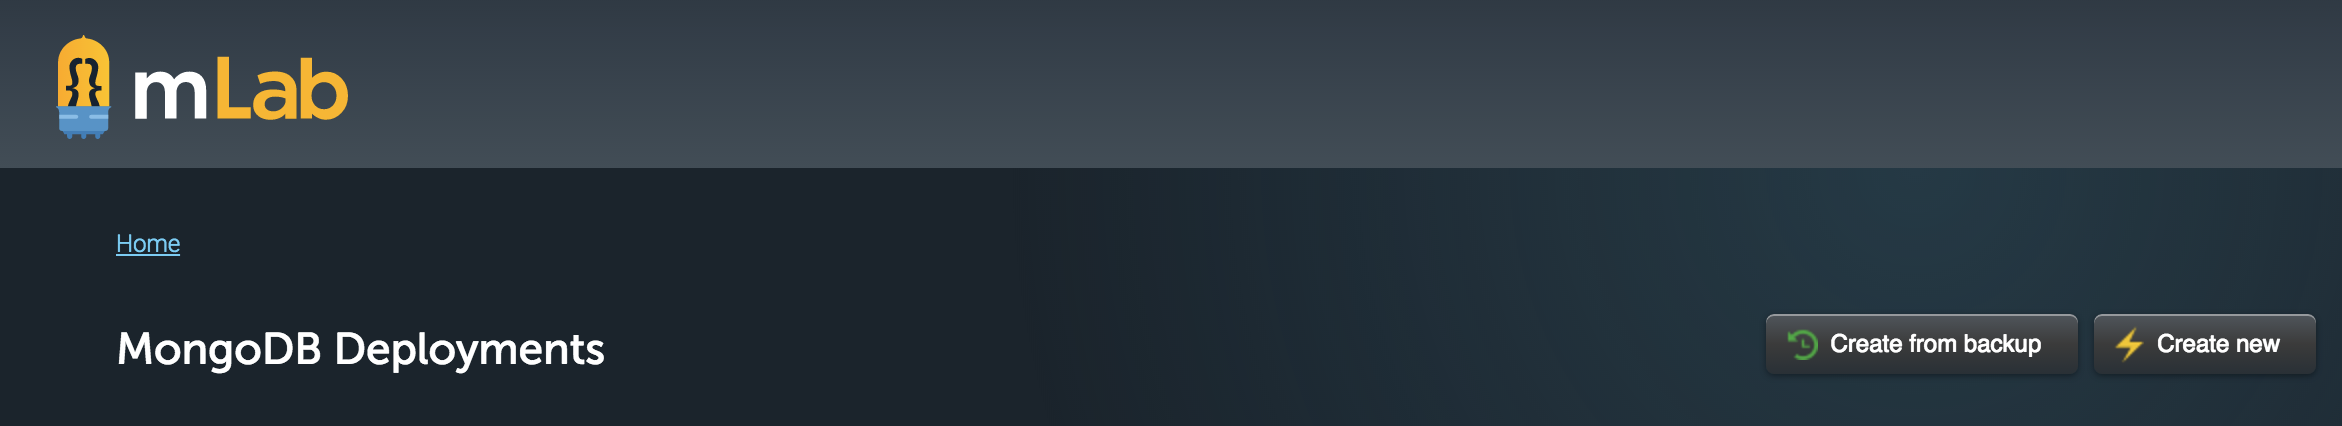
\includegraphics[width=0.85\textwidth]{images/mlab_controlpanel}
\caption{}
\label{fig:}
\end{figure}

\paragraph{} Click the ``Create new'' button. Now choose the single-node tab uder \emph{Plan} to reveal the free \emph{sandbox} option.

\begin{figure}[H]
\centering
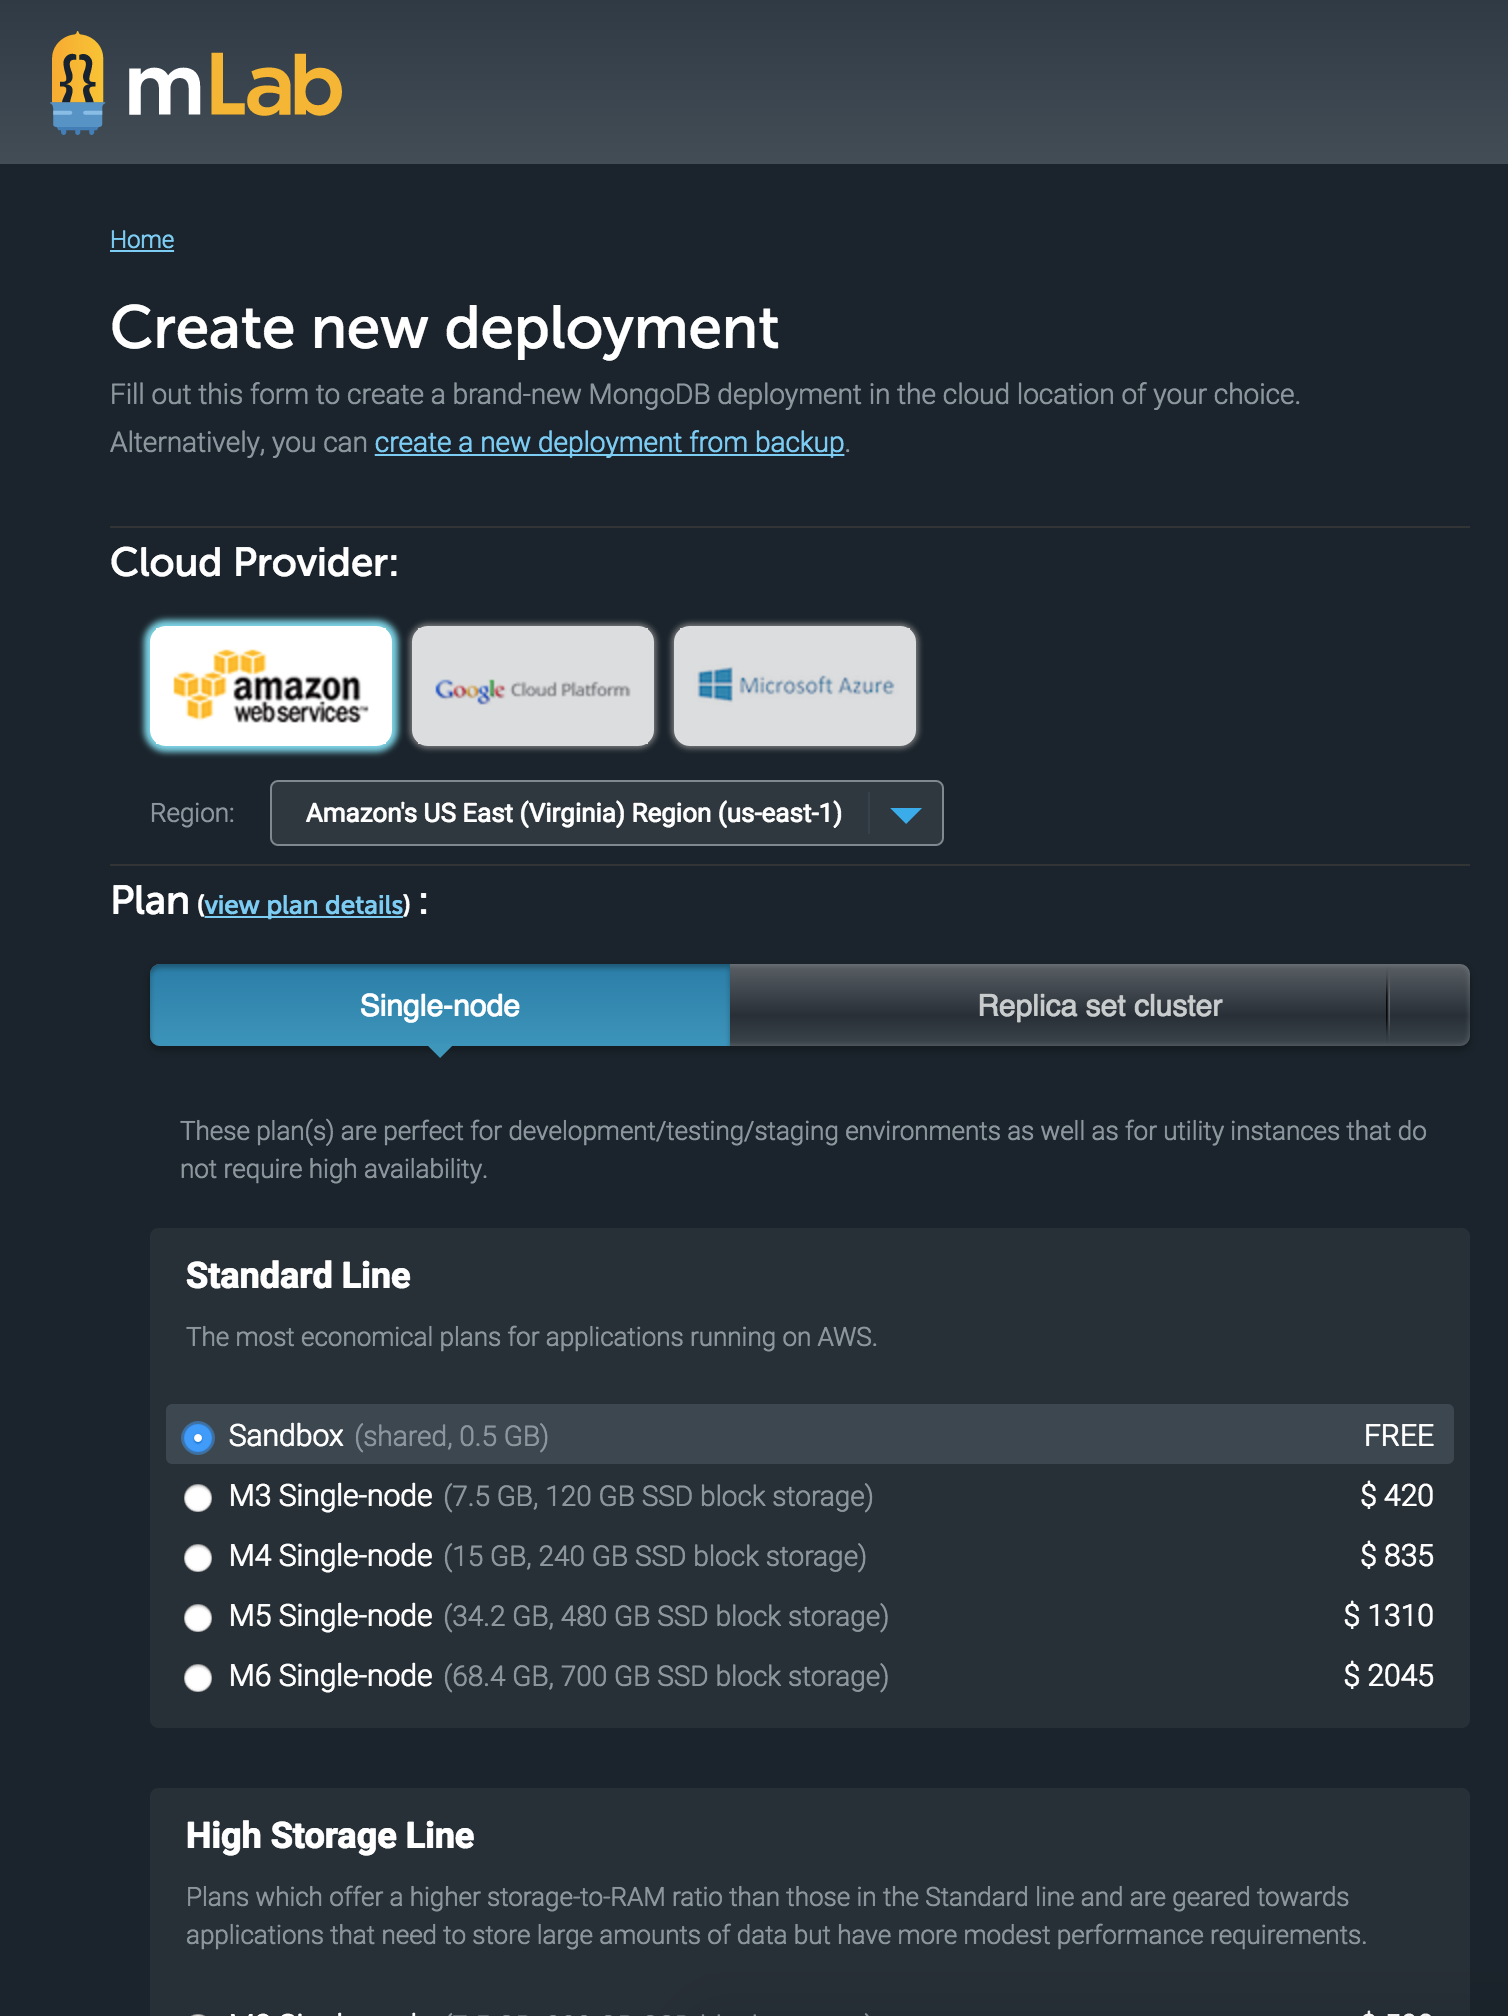
\includegraphics[width=0.85\textwidth]{images/mlab_newdeployment}
\caption{}
\label{fig:}
\end{figure}

\paragraph{} Give your new database a name then click ``Create new MongoDB deployment''

\begin{figure}[H]
\centering
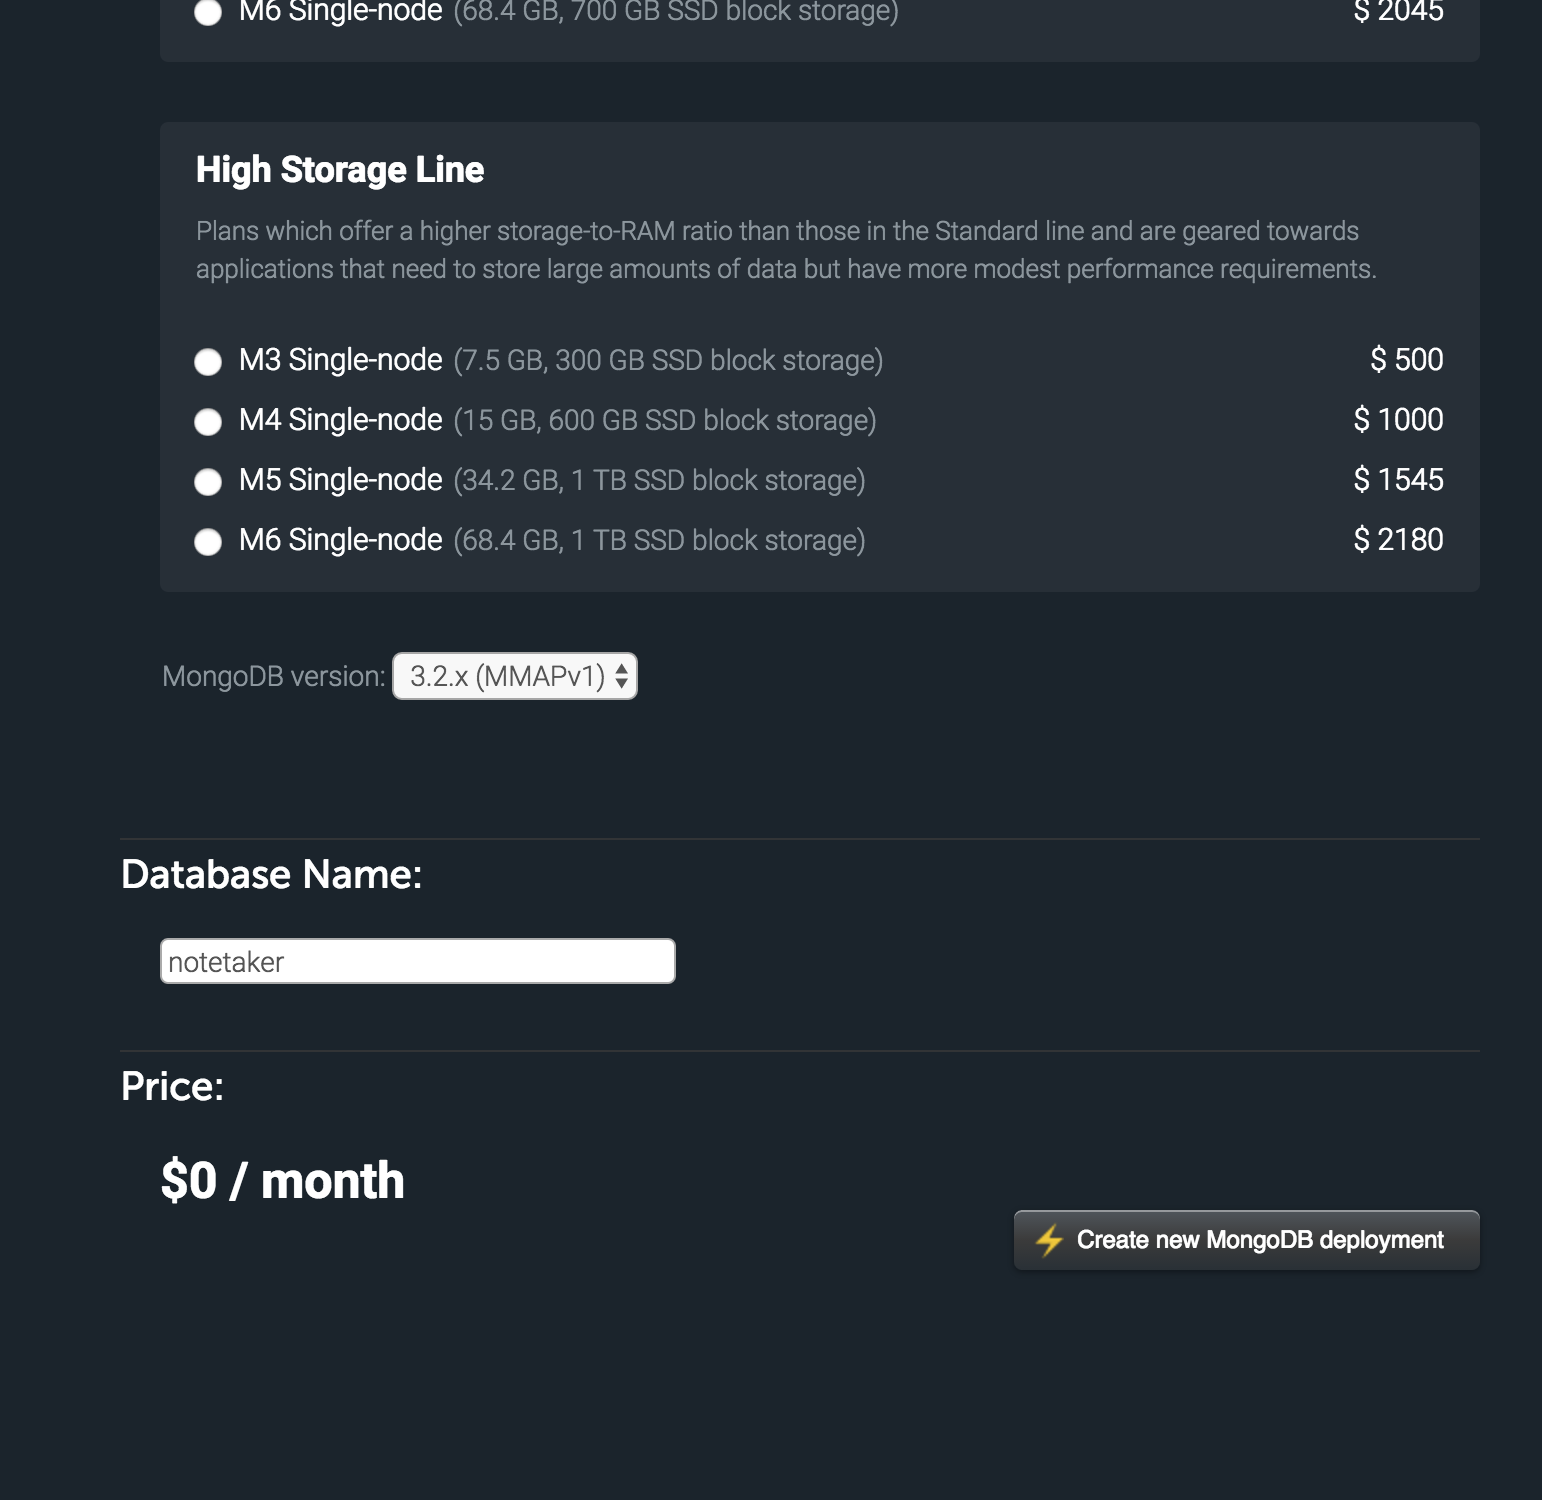
\includegraphics[width=0.85\textwidth]{images/mlab_dbname}
\caption{}
\label{fig:}
\end{figure}

\paragraph{} Think of a MongoDB, for now, as a collection of collections. So we need to name a default collection to insert data into. Click the ``+ Add collection'' button, then type in a name for the collection, e.g. ``'notes''.

\begin{figure}[H]
\centering
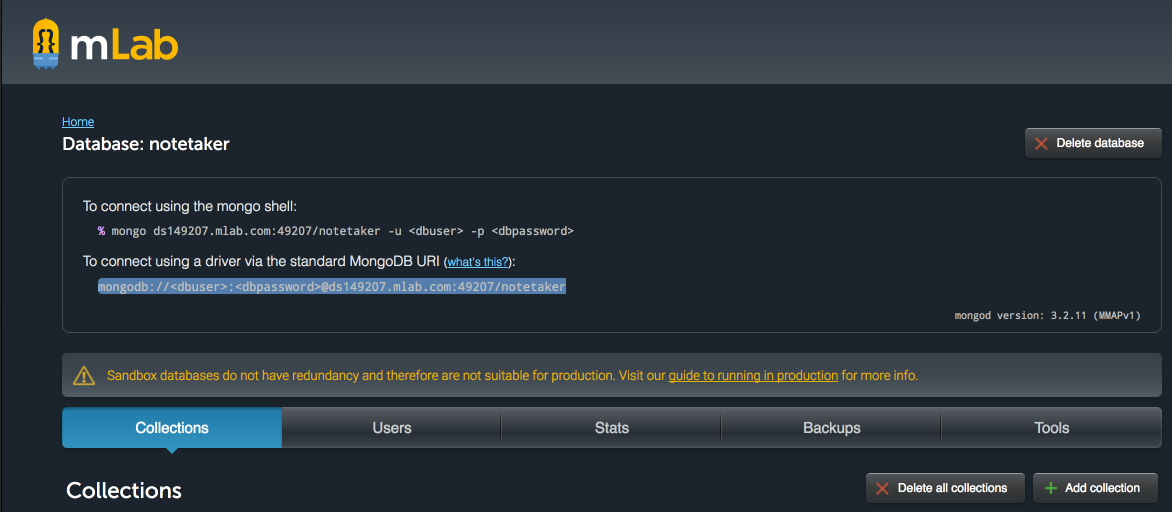
\includegraphics[width=0.85\textwidth]{images/mlab_mongocollection}
\caption{}
\label{fig:}
\end{figure}

\paragraph{} On the database page, mLab gives you connection details for your collection on the database page, e.g.

\begin{framed}
    mongodb://<dbuser>:<dbpassword>@dsxxxxxx.mlab.com:49207/notetaker
\end{framed}

\paragraph{} We still need a username and password however, so we need to create a user by clicking the ``'Add database user'' button and entering a username and password.

\begin{figure}[H]
\centering
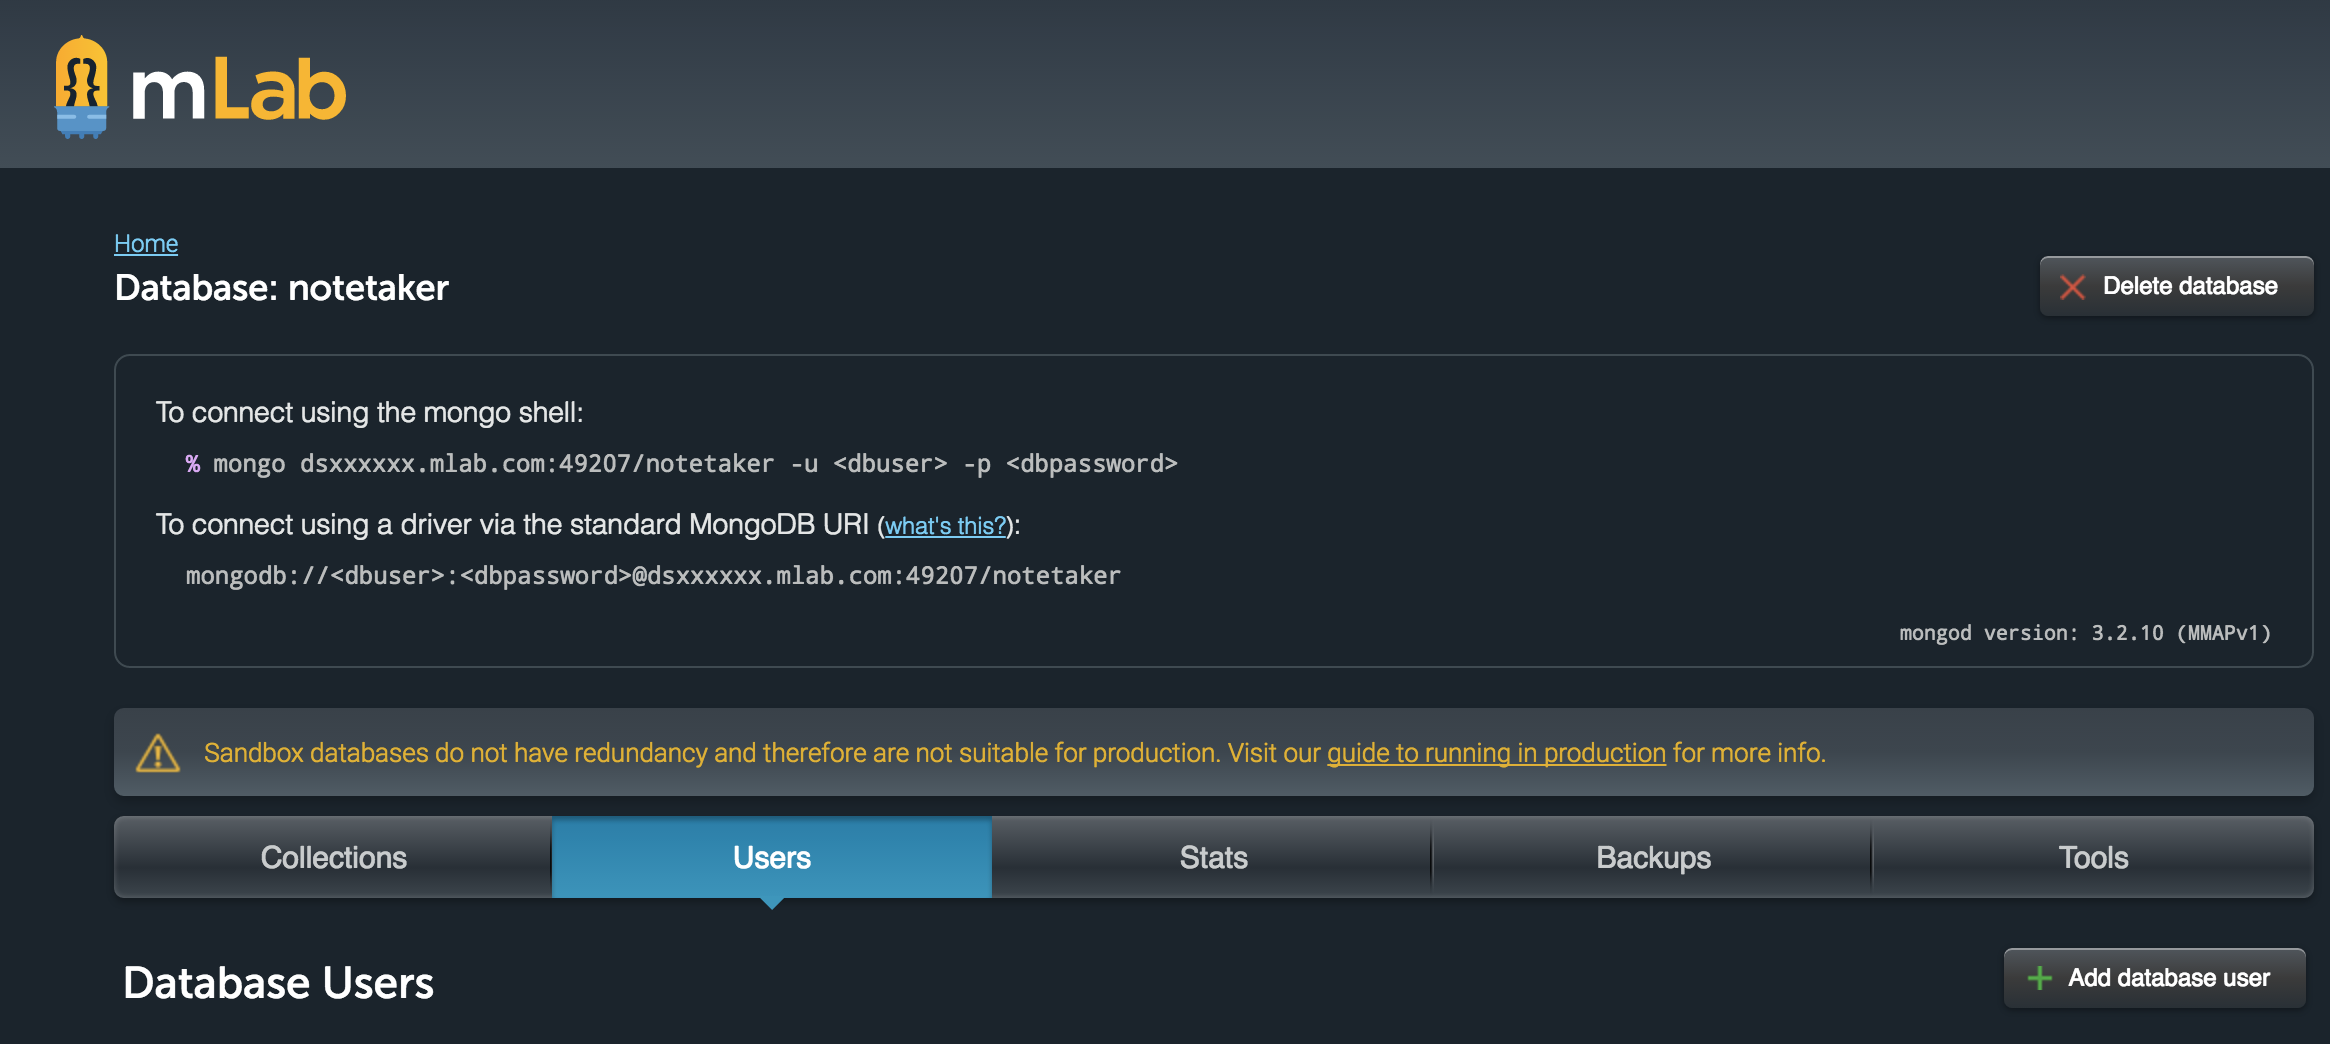
\includegraphics[width=0.85\textwidth]{images/mlab_dbinfo}
\caption{}
\label{fig:}
\end{figure}

\paragraph{} You should now be able to connect to your database from node. First install a MongoDB package using npm, e.g. 

\begin{lstlisting}[style=DOS]
    npm install mongodb
\end{lstlisting}

\paragraph{} We can now access our mLab instance of a Mongo database using JavaScript within a node app as indicated in the following fragment:

\begin{lstlisting}
const MongoClient = require('mongodb').MongoClient;

const MONGO_URL = 'YOUR_URL_HERE';

MongoClient.connect(MONGO_URL, (err, db) => {  
  if (err) {
    return console.log(err);
  }

  // Do something with db here, like inserting a record
  db.collection('notes').insertOne(
    {
      title: 'Hello MongoDB',
      text: 'Hopefully this works!'
    },
    function (err, res) {
      if (err) {
        db.close();
        return console.log(err);
      }
      // Success
      db.close();
    }
  )
});
\end{lstlisting}

\paragraph{} Obviously there's a whole lot more that MongoDB and mLab can do, but that is what documentation is for. Perhaps a first exercise might be to reimplement the hit counter app that we used in filesystem and sql persistence to use a Mongo instance instead?

\subsection{Challenges}
\paragraph{} You should consider how to incorporate appropriate data storage into the sites that we've already developed during previous challenges. For example, if you've been working on the dungeon-crawler game then cookies are a really good, light-weight method of storing a small amount of data about the current player. For example, the players health, what they are carrying, which locations they've visited. Obviously, you have a small amount of space to store your data in a cookie, but this should be more than sufficient for simple player specific data. If you are generating a larger dungeon, then you might want to consider using one of the other types of client-side storage. The nice thing about this approach is that each time your player revisits the site they should be able to pick up at exactly the place that they left off. This is a nice way to persist a game whilst maintaining a very lightweight, casula approach for your player.
\end{document}

%\begin{framed}
%\end{framed}


%\begin{lstlisting}
%\end{lstlisting}

%\begin{lstlisting}[style=DOS]
%\end{lstlisting}
